\documentclass[twoside]{book}

% Packages required by doxygen
\usepackage{fixltx2e}
\usepackage{calc}
\usepackage{doxygen}
\usepackage{graphicx}
\usepackage[utf8]{inputenc}
\usepackage{makeidx}
\usepackage{multicol}
\usepackage{multirow}
\PassOptionsToPackage{warn}{textcomp}
\usepackage{textcomp}
\usepackage[nointegrals]{wasysym}
\usepackage[table]{xcolor}

% Font selection
\usepackage[T1]{fontenc}
\usepackage{mathptmx}
\usepackage[scaled=.90]{helvet}
\usepackage{courier}
\usepackage{amssymb}
\usepackage{sectsty}
\renewcommand{\familydefault}{\sfdefault}
\allsectionsfont{%
  \fontseries{bc}\selectfont%
  \color{darkgray}%
}
\renewcommand{\DoxyLabelFont}{%
  \fontseries{bc}\selectfont%
  \color{darkgray}%
}
\newcommand{\+}{\discretionary{\mbox{\scriptsize$\hookleftarrow$}}{}{}}

% Page & text layout
\usepackage{geometry}
\geometry{%
  a4paper,%
  top=2.5cm,%
  bottom=2.5cm,%
  left=2.5cm,%
  right=2.5cm%
}
\tolerance=750
\hfuzz=15pt
\hbadness=750
\setlength{\emergencystretch}{15pt}
\setlength{\parindent}{0cm}
\setlength{\parskip}{0.2cm}
\makeatletter
\renewcommand{\paragraph}{%
  \@startsection{paragraph}{4}{0ex}{-1.0ex}{1.0ex}{%
    \normalfont\normalsize\bfseries\SS@parafont%
  }%
}
\renewcommand{\subparagraph}{%
  \@startsection{subparagraph}{5}{0ex}{-1.0ex}{1.0ex}{%
    \normalfont\normalsize\bfseries\SS@subparafont%
  }%
}
\makeatother

% Headers & footers
\usepackage{fancyhdr}
\pagestyle{fancyplain}
\fancyhead[LE]{\fancyplain{}{\bfseries\thepage}}
\fancyhead[CE]{\fancyplain{}{}}
\fancyhead[RE]{\fancyplain{}{\bfseries\leftmark}}
\fancyhead[LO]{\fancyplain{}{\bfseries\rightmark}}
\fancyhead[CO]{\fancyplain{}{}}
\fancyhead[RO]{\fancyplain{}{\bfseries\thepage}}
\fancyfoot[LE]{\fancyplain{}{}}
\fancyfoot[CE]{\fancyplain{}{}}
\fancyfoot[RE]{\fancyplain{}{\bfseries\scriptsize Generated on Tue Feb 21 2017 22\+:18\+:05 for My Project by Doxygen }}
\fancyfoot[LO]{\fancyplain{}{\bfseries\scriptsize Generated on Tue Feb 21 2017 22\+:18\+:05 for My Project by Doxygen }}
\fancyfoot[CO]{\fancyplain{}{}}
\fancyfoot[RO]{\fancyplain{}{}}
\renewcommand{\footrulewidth}{0.4pt}
\renewcommand{\chaptermark}[1]{%
  \markboth{#1}{}%
}
\renewcommand{\sectionmark}[1]{%
  \markright{\thesection\ #1}%
}

% Indices & bibliography
\usepackage{natbib}
\usepackage[titles]{tocloft}
\setcounter{tocdepth}{3}
\setcounter{secnumdepth}{5}
\makeindex

% Hyperlinks (required, but should be loaded last)
\usepackage{ifpdf}
\ifpdf
  \usepackage[pdftex,pagebackref=true]{hyperref}
\else
  \usepackage[ps2pdf,pagebackref=true]{hyperref}
\fi
\hypersetup{%
  colorlinks=true,%
  linkcolor=blue,%
  citecolor=blue,%
  unicode%
}

% Custom commands
\newcommand{\clearemptydoublepage}{%
  \newpage{\pagestyle{empty}\cleardoublepage}%
}


%===== C O N T E N T S =====

\begin{document}

% Titlepage & ToC
\hypersetup{pageanchor=false,
             bookmarks=true,
             bookmarksnumbered=true,
             pdfencoding=unicode
            }
\pagenumbering{roman}
\begin{titlepage}
\vspace*{7cm}
\begin{center}%
{\Large My Project }\\
\vspace*{1cm}
{\large Generated by Doxygen 1.8.8}\\
\vspace*{0.5cm}
{\small Tue Feb 21 2017 22:18:05}\\
\end{center}
\end{titlepage}
\clearemptydoublepage
\tableofcontents
\clearemptydoublepage
\pagenumbering{arabic}
\hypersetup{pageanchor=true}

%--- Begin generated contents ---
\chapter{Hierarchical Index}
\section{Class Hierarchy}
This inheritance list is sorted roughly, but not completely, alphabetically\+:\begin{DoxyCompactList}
\item \contentsline{section}{Client}{\pageref{classClient}}{}
\item J\+Frame\begin{DoxyCompactList}
\item \contentsline{section}{Myframe}{\pageref{classMyframe}}{}
\end{DoxyCompactList}
\end{DoxyCompactList}

\chapter{Class Index}
\section{Class List}
Here are the classes, structs, unions and interfaces with brief descriptions\+:\begin{DoxyCompactList}
\item\contentsline{section}{\hyperlink{structcppu_1_1TCPServer_1_1Callback}{cppu\+::\+T\+C\+P\+Server\+::\+Callback} \\*\hyperlink{structcppu_1_1TCPServer_1_1Callback}{Callback} interface }{\pageref{structcppu_1_1TCPServer_1_1Callback}}{}
\item\contentsline{section}{\hyperlink{structcppu_1_1TCPServer_1_1CallbackMethod}{cppu\+::\+T\+C\+P\+Server\+::\+Callback\+Method$<$ T $>$} }{\pageref{structcppu_1_1TCPServer_1_1CallbackMethod}}{}
\item\contentsline{section}{\hyperlink{classFactory}{Factory} }{\pageref{classFactory}}{}
\item\contentsline{section}{\hyperlink{classFilm}{Film} }{\pageref{classFilm}}{}
\item\contentsline{section}{\hyperlink{structcppu_1_1InputBuffer}{cppu\+::\+Input\+Buffer} }{\pageref{structcppu_1_1InputBuffer}}{}
\item\contentsline{section}{\hyperlink{classListMedia}{List\+Media$<$ T $>$} }{\pageref{classListMedia}}{}
\item\contentsline{section}{\hyperlink{classMultimedia}{Multimedia} }{\pageref{classMultimedia}}{}
\item\contentsline{section}{\hyperlink{classMyBase}{My\+Base} }{\pageref{classMyBase}}{}
\item\contentsline{section}{\hyperlink{classPhoto}{Photo} }{\pageref{classPhoto}}{}
\item\contentsline{section}{\hyperlink{classcppu_1_1ServerSocket}{cppu\+::\+Server\+Socket} \\*T\+C\+P/\+I\+P server socket. This class implements a T\+C\+P/\+I\+P socket that waits for requests to come in over the network. A\+F\+\_\+\+I\+N\+E\+T connections following the I\+Pv4 Internet protocol are supported }{\pageref{classcppu_1_1ServerSocket}}{}
\item\contentsline{section}{\hyperlink{classcppu_1_1Socket}{cppu\+::\+Socket} \\*T\+C\+P/\+I\+P or U\+D\+P/\+Datagram socket. This class encapsulates a T\+C\+P/\+I\+P or U\+D\+P/\+Datagram socket. A\+F\+\_\+\+I\+N\+E\+T connections following the I\+Pv4 Internet protocol are supported }{\pageref{classcppu_1_1Socket}}{}
\item\contentsline{section}{\hyperlink{classcppu_1_1SocketBuffer}{cppu\+::\+Socket\+Buffer} \\*Preserves record boundaries when exchanging data between connected T\+C\+P/\+I\+P sockets. This class ensures that one call to \hyperlink{classcppu_1_1SocketBuffer_a92ae0351aaee8719d34e8c4618495d59}{write\+Line()} corresponds to one and exactly one call to \hyperlink{classcppu_1_1SocketBuffer_a222769d3776b9cbd3a727ee1f0e60358}{read\+Line()} on the other side. This differs from the behavior of \hyperlink{classcppu_1_1Socket_aeac77f859159715e2d63a5a0dc118788}{Socket\+::send()} and \hyperlink{classcppu_1_1Socket_a37c382af52cc02f92c0e19a0c6e0e04f}{Socket\+::receive()} because T\+C\+P/\+I\+P connected sockets do not preserve record boundaries. \hyperlink{classcppu_1_1SocketBuffer_a92ae0351aaee8719d34e8c4618495d59}{write\+Line()} and \hyperlink{classcppu_1_1SocketBuffer_a222769d3776b9cbd3a727ee1f0e60358}{read\+Line()} solve this problem by automatically adding and searching for a separator between successive lines }{\pageref{classcppu_1_1SocketBuffer}}{}
\item\contentsline{section}{\hyperlink{classcppu_1_1TCPConnection}{cppu\+::\+T\+C\+P\+Connection} \\*Connection with a given client. Each \hyperlink{classcppu_1_1TCPConnection}{T\+C\+P\+Connection} uses a different thread }{\pageref{classcppu_1_1TCPConnection}}{}
\item\contentsline{section}{\hyperlink{classcppu_1_1TCPLock}{cppu\+::\+T\+C\+P\+Lock} \\*Locks the server in read mode or in write mode. Must be created {\itshape in the stack} by the callback method }{\pageref{classcppu_1_1TCPLock}}{}
\item\contentsline{section}{\hyperlink{classcppu_1_1TCPServer}{cppu\+::\+T\+C\+P\+Server} \\*T\+C\+P/\+I\+P I\+Pv4 server. The server supports T\+C\+P/\+I\+P A\+F\+\_\+\+I\+N\+E\+T connections (following the I\+Pv4 Internet protocol) with multiple clients. One thread is used per client }{\pageref{classcppu_1_1TCPServer}}{}
\item\contentsline{section}{\hyperlink{classVideo}{Video} }{\pageref{classVideo}}{}
\end{DoxyCompactList}

\chapter{Class Documentation}
\hypertarget{classClient}{\section{Client Class Reference}
\label{classClient}\index{Client@{Client}}
}
\subsection*{Public Member Functions}
\begin{DoxyCompactItemize}
\item 
\hyperlink{classClient_a163113b9c3fda23dcdc750db9278afbe}{Client} (String host, int port)  throws Unknown\+Host\+Exception, I\+O\+Exception 
\item 
String \hyperlink{classClient_ab26831c395da92b5893066f9ce7963a4}{send} (String request)
\end{DoxyCompactItemize}
\subsection*{Static Public Member Functions}
\begin{DoxyCompactItemize}
\item 
static void \hyperlink{classClient_ac9fec818083d641b633a8e4a75d981a7}{main} (String argv\mbox{[}$\,$\mbox{]})
\end{DoxyCompactItemize}


\subsection{Constructor \& Destructor Documentation}
\hypertarget{classClient_a163113b9c3fda23dcdc750db9278afbe}{\index{Client@{Client}!Client@{Client}}
\index{Client@{Client}!Client@{Client}}
\subsubsection[{Client}]{\setlength{\rightskip}{0pt plus 5cm}Client.\+Client (
\begin{DoxyParamCaption}
\item[{String}]{host, }
\item[{int}]{port}
\end{DoxyParamCaption}
) throws Unknown\+Host\+Exception, I\+O\+Exception\hspace{0.3cm}{\ttfamily [inline]}}}\label{classClient_a163113b9c3fda23dcdc750db9278afbe}
Initialise la connexion. Renvoie une exception en cas d'erreur. 

\subsection{Member Function Documentation}
\hypertarget{classClient_ac9fec818083d641b633a8e4a75d981a7}{\index{Client@{Client}!main@{main}}
\index{main@{main}!Client@{Client}}
\subsubsection[{main}]{\setlength{\rightskip}{0pt plus 5cm}static void Client.\+main (
\begin{DoxyParamCaption}
\item[{String}]{argv\mbox{[}$\,$\mbox{]}}
\end{DoxyParamCaption}
)\hspace{0.3cm}{\ttfamily [inline]}, {\ttfamily [static]}}}\label{classClient_ac9fec818083d641b633a8e4a75d981a7}
Lit une requete depuis le Terminal, envoie cette requete au serveur, recupere sa reponse et l'affiche sur le Terminal. Noter que le programme bloque si le serveur ne repond pas. \hypertarget{classClient_ab26831c395da92b5893066f9ce7963a4}{\index{Client@{Client}!send@{send}}
\index{send@{send}!Client@{Client}}
\subsubsection[{send}]{\setlength{\rightskip}{0pt plus 5cm}String Client.\+send (
\begin{DoxyParamCaption}
\item[{String}]{request}
\end{DoxyParamCaption}
)\hspace{0.3cm}{\ttfamily [inline]}}}\label{classClient_ab26831c395da92b5893066f9ce7963a4}
Envoie une requete au server et retourne sa reponse. Noter que la methode bloque si le serveur ne repond pas. 

The documentation for this class was generated from the following file\+:\begin{DoxyCompactItemize}
\item 
Client.\+java\end{DoxyCompactItemize}

\hypertarget{classMyframe}{\section{Myframe Class Reference}
\label{classMyframe}\index{Myframe@{Myframe}}
}


Inheritance diagram for Myframe\+:
\nopagebreak
\begin{figure}[H]
\begin{center}
\leavevmode
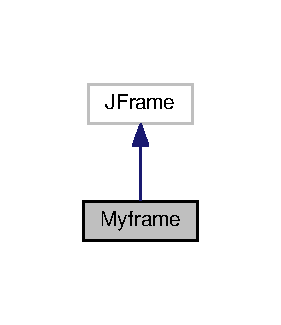
\includegraphics[width=135pt]{classMyframe__inherit__graph}
\end{center}
\end{figure}


Collaboration diagram for Myframe\+:
\nopagebreak
\begin{figure}[H]
\begin{center}
\leavevmode
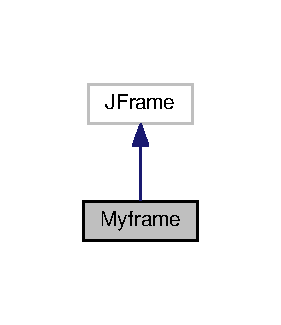
\includegraphics[width=135pt]{classMyframe__coll__graph}
\end{center}
\end{figure}
\subsection*{Public Member Functions}
\begin{DoxyCompactItemize}
\item 
\hyperlink{classMyframe_ad618e4bee9255c02d0631105ac559580}{Myframe} ()
\begin{DoxyCompactList}\small\item\em \hyperlink{classMyframe}{Myframe}. \end{DoxyCompactList}\item 
String \hyperlink{classMyframe_a6f872a5cc73cdfd73ced1615009e5a7c}{get\+\_\+request} ()
\begin{DoxyCompactList}\small\item\em get\+\_\+request \end{DoxyCompactList}\item 
void \hyperlink{classMyframe_a024aeca2f82fd2ff80889f620804de1d}{send} (String request)
\begin{DoxyCompactList}\small\item\em send \end{DoxyCompactList}\item 
void \hyperlink{classMyframe_ae55afc91e2f0397f701d39d40907057c}{init\+\_\+layout} ()
\begin{DoxyCompactList}\small\item\em init\+\_\+layout \end{DoxyCompactList}\end{DoxyCompactItemize}
\subsection*{Static Public Member Functions}
\begin{DoxyCompactItemize}
\item 
\hypertarget{classMyframe_ac550acb95f01d6163f6db51f32e614d8}{static void {\bfseries main} (String\mbox{[}$\,$\mbox{]} args)}\label{classMyframe_ac550acb95f01d6163f6db51f32e614d8}

\end{DoxyCompactItemize}


\subsection{Constructor \& Destructor Documentation}
\hypertarget{classMyframe_ad618e4bee9255c02d0631105ac559580}{\index{Myframe@{Myframe}!Myframe@{Myframe}}
\index{Myframe@{Myframe}!Myframe@{Myframe}}
\subsubsection[{Myframe}]{\setlength{\rightskip}{0pt plus 5cm}Myframe.\+Myframe (
\begin{DoxyParamCaption}
{}
\end{DoxyParamCaption}
)\hspace{0.3cm}{\ttfamily [inline]}}}\label{classMyframe_ad618e4bee9255c02d0631105ac559580}


\hyperlink{classMyframe}{Myframe}. 


\begin{DoxyParams}{Parameters}
{\em } & return  Construct the class \hyperlink{classMyframe}{Myframe}. initialize the client \\
\hline
\end{DoxyParams}


\subsection{Member Function Documentation}
\hypertarget{classMyframe_a6f872a5cc73cdfd73ced1615009e5a7c}{\index{Myframe@{Myframe}!get\+\_\+request@{get\+\_\+request}}
\index{get\+\_\+request@{get\+\_\+request}!Myframe@{Myframe}}
\subsubsection[{get\+\_\+request}]{\setlength{\rightskip}{0pt plus 5cm}String Myframe.\+get\+\_\+request (
\begin{DoxyParamCaption}
{}
\end{DoxyParamCaption}
)\hspace{0.3cm}{\ttfamily [inline]}}}\label{classMyframe_a6f872a5cc73cdfd73ced1615009e5a7c}


get\+\_\+request 


\begin{DoxyParams}{Parameters}
{\em } & return request  According to the input of user, set the value of request and return it. \\
\hline
\end{DoxyParams}
\hypertarget{classMyframe_ae55afc91e2f0397f701d39d40907057c}{\index{Myframe@{Myframe}!init\+\_\+layout@{init\+\_\+layout}}
\index{init\+\_\+layout@{init\+\_\+layout}!Myframe@{Myframe}}
\subsubsection[{init\+\_\+layout}]{\setlength{\rightskip}{0pt plus 5cm}void Myframe.\+init\+\_\+layout (
\begin{DoxyParamCaption}
{}
\end{DoxyParamCaption}
)\hspace{0.3cm}{\ttfamily [inline]}}}\label{classMyframe_ae55afc91e2f0397f701d39d40907057c}


init\+\_\+layout 


\begin{DoxyParams}{Parameters}
{\em } & return  initialize the layout. The total layout is Box\+Layout. The part of input uses Grid\+Layout. \\
\hline
\end{DoxyParams}
\hypertarget{classMyframe_a024aeca2f82fd2ff80889f620804de1d}{\index{Myframe@{Myframe}!send@{send}}
\index{send@{send}!Myframe@{Myframe}}
\subsubsection[{send}]{\setlength{\rightskip}{0pt plus 5cm}void Myframe.\+send (
\begin{DoxyParamCaption}
\item[{String}]{request}
\end{DoxyParamCaption}
)\hspace{0.3cm}{\ttfamily [inline]}}}\label{classMyframe_a024aeca2f82fd2ff80889f620804de1d}


send 


\begin{DoxyParams}{Parameters}
{\em request} & \\
\hline
\end{DoxyParams}
\begin{DoxyReturn}{Returns}
According to the input of user, set the value of request and return it. 
\end{DoxyReturn}


The documentation for this class was generated from the following file\+:\begin{DoxyCompactItemize}
\item 
Myframe.\+java\end{DoxyCompactItemize}

%--- End generated contents ---

% Index
\newpage
\phantomsection
\addcontentsline{toc}{chapter}{Index}
\printindex

\end{document}
